\documentclass[11pt]{scrartcl}

\title{Software Architektur: JBomberman}
\author{Silvan Adrian \\ Fabian Binna \\ Pascal Kistler}
\date{\today{}}

\usepackage[ngerman]{babel}
\usepackage[automark]{scrpage2}
\usepackage{hyperref}
\usepackage{color}
\usepackage[normalem]{ulem}
\usepackage{scrpage2}
\usepackage{graphicx}
\usepackage{tabularx}
\usepackage{lscape}
\graphicspath{ {./images/} }
\pagestyle{scrheadings}

\clearscrheadfoot
\ihead{
\includegraphics[scale=0.4]{jbomberman}}
\ohead{Projekt: JBomberman}
\ifoot{Software Architektur: JBomberman}
\cfoot{Version: 1.18}
\ofoot{Datum: 24.05.15}
\setheadsepline{0.5pt}
\setfootsepline{0.5pt}

\usepackage{ucs}
\usepackage[utf8x]{inputenc}
\usepackage[T1]{fontenc}


\begin{document}
\def\arraystretch{1.5}
\begin{titlepage}
\begin{center}
\vspace{10em}

\includegraphics[scale=2]{jbomberman}
\vspace{10em}
\end{center}
\begin{center}
\huge {Projekt: JBomberman} \\
\huge {Software Architektur}
\end{center}
\begin{center}
\vspace{10em}
\LARGE {Pascal Kistler} \\
\LARGE {Silvan Adrian} \\
\LARGE {Fabian Binna}
\end{center}

\end{titlepage}

\newpage
\section{Änderungshistorie}
\label{sec:Änderungen}

\begin{tabularx}{\linewidth}{l l X l}
\textbf{Datum} & \textbf{Version} & \textbf{Änderung}  & \textbf{Autor} \\
\hline
\textbf{01.04.15} & 1.00 & Erstellung des Dokuments & Gruppe \\
\textbf{04.04.15} & 1.01 & Logische Architektur & Fabian Binna \\
\textbf{05.04.15} & 1.02 & Logische Architektur Client & Fabian Binna\\
\textbf{05.04.15} & 1.03 & Ziele und Einschränkungen & Silvan Adrian\\
\textbf{06.04.15} & 1.04 & Logische Architektur Server & Fabian Binna\\
\textbf{06.04.15} & 1.05 & Zustandsdiagramm Workflows & Fabian Binna\\
\textbf{06.04.15} & 1.06 & Systemübersicht Grafik und Beschreibung & Silvan Adrian\\
\textbf{06.04.15} & 1.07 & Schnittstellen & Fabian Binna\\
\textbf{06.04.15} & 1.08 & Grössen und Leistung + Externes Design & Silvan Adrian\\
\textbf{07.04.15} & 1.09 & Datenübertragung & Fabian Binna\\
\textbf{07.04.15} & 1.10 & Prozesse und Threads & Fabian Binna\\
\textbf{07.04.15} & 1.11 & Korrekturen & Fabian Binna\\
\textbf{07.04.15} & 1.12 & Korrekturen & Silvan Adrian\\
\textbf{16.04.15} & 1.13 & Sequenz Diagramm Action & Fabian Binna\\
\textbf{05.05.15} & 1.14 & Anpassungen & Fabian Binna\\
\bf{05.05.15} & 1.15 & Anpassungen an Client-, ServerController und LobbyCommunication 
& Pascal Kistler\\
\bf{06.05.15} & 1.16 & Externes Design erweitert + Grössen Leistung angepasst & Silvan Adrian\\
\bf{16.05.15} & 1.17 & NetworkFacade und LobbyCommunication angepasst & Pascal Kistler\\
\bf{24.05.15} & 1.18 & Packagediagramme angepasst & Pascal Kistler\\
\end{tabularx}

\newpage
\tableofcontents
\newpage

\section{Einführung}
\subsection{Zweck}
Dieses Dokument beschreibt die Software Architektur für das Projekt JBomberman.
\subsection{Gültigkeitsbereich}
Dieses Dokument ist während des ganzen Projekts gültig und wird laufend aktualisiert.
\subsection{Referenzen}
\subsection{Übersicht}
Die LogischeSicht wurde in drei Teile unterteilt: Applikationsübergreifend, Client und Server. Die Schnittstellen werden anhand einer kompletten Packageübersicht gezeigt. Im Kapitel Datenübertragung wird auf die RabbitMQ-Technologie eingegangen. 
\subsubsection{Glossar}
Siehe Dokument Glossar.pdf
 
\section{Systemübersicht}
JBomberman kann nur als Mehrspielerspiel gespielt werden, daher wird immer ein verfügbarer Server benötigt + muss ein RabbitMQ Server verfügbar sein.
Zudem braucht es mindestens 2 Clients, damit ein Spiel überhaupt gespielt werden kann.
Zur Veranschaulichung der Austausch zwischen 2 Clients und 1 Server:

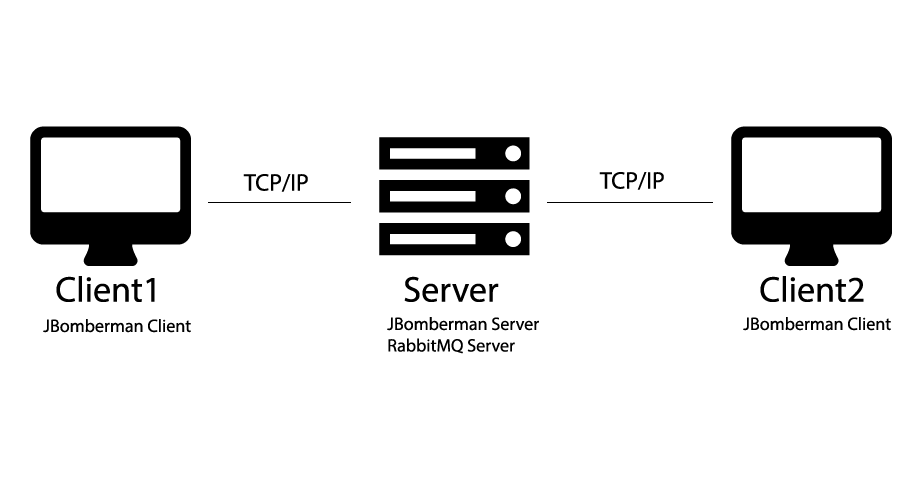
\includegraphics[scale=0.45]{systemuebersicht}
\newpage

 
\section{Architektonische Ziele \& Einschränkungen}
\subsection{Ziele}
\begin{itemize}
    \item Die Spielumgebungen müssen mit allen Clients synchronisiert werden (über den dedizierten Server)
    \item Möglichkeit weitere PowerUp's einzubauen.
    \item Austausch zwischen den Clients und dem Server wird über JMS umgesetzt.
\end{itemize}


\subsection{Einschränkungen}
\begin{itemize}
    \item Es wird keinen Live Server geben, jeder der das Spiel spielen will muss einen eigenen Server starten.
    \item Die Clients können nur zum Server Verbindung aufnehmen, wenn diese die IP des Servers kennen.
\end{itemize}


\newpage
 
\section{Logische Architektur: Applikationsübergreifend}
Dieses Package Diagramm zeigt sowohl Client, als auch Server. Client und Server sind zwei eigenständige Applikationen, die getrennt ausgeführt werden. Sie verwenden jedoch teilweise die gleichen Packages.

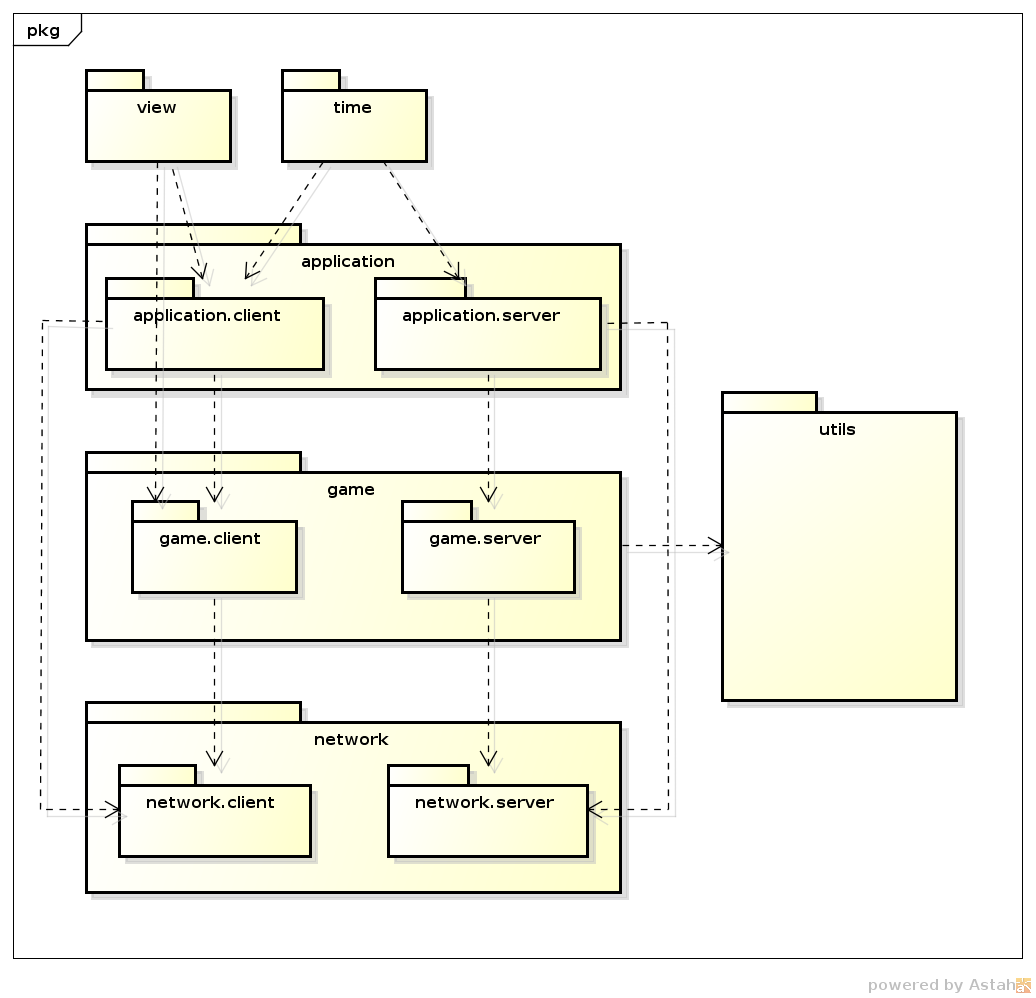
\includegraphics[scale=0.5]{LogischeSicht}

\newpage

\subsection{Domain/game}
Im Package game befinden sich Klassen und Interfaces, die von Server und Client gemeinsam genutzt werden.
\subsubsection{Klassenstruktur}
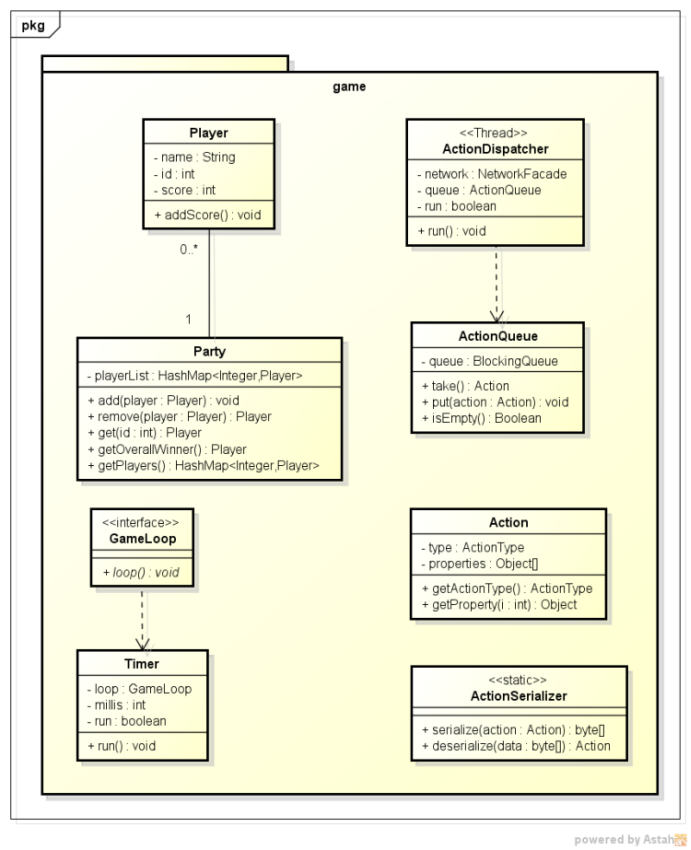
\includegraphics[scale=0.75]{ClassDiagramGame}
\newpage
\textbf{Action}\\
Die Action Klasse wird über das Netzwerk zwischen Server und Client versendet und enthält Statusnachrichten, sowie Aktualisierungsdaten für die Objekte.\\

\textbf{ActionQueue}\\
Die ActionQueue speichert die Actions. Die Actions werden bei jedem loop aus der Queue entfernt und verarbeitet. Die ActionQueue muss Threadsafe sein, da der ActionDispatcher die Queue füllt.\\

\textbf{ActionDispatcher}\\
Der ActionDispatcher ist ein Thread und ist ausschliesslich damit beschäftig auf eingehende Messages zu warten und diese als Action in der Queue einzureihen.\\

\textbf{Player}\\
Der Player speichert die Daten eines Spielers. Die Daten werden für die Zuweisung von Actions und das Darstellen des Scoreboard benötigt.\\

\textbf{Party}\\
Die Party beinhaltet alle Player eines Spiels. Ein Spiel kann nur mittels einer Party instanziert werden.

\newpage

\subsection{Utilities/utils}
Im Package utils befinden sich Hilfsklassen.
\subsubsection{Klassenstruktur}
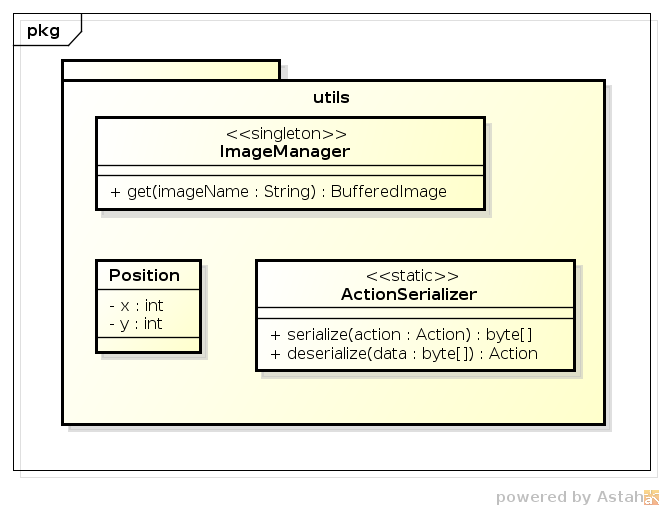
\includegraphics[scale=0.75]{ClassDiagramUtils}

\textbf{ImageManager}\\
Der ImageManager lädt die Bilder. Jedes Sprite holt sich von da die Bilddaten.\\

\textbf{ActionSerializer}\\
Die Methoden des ActionSerializer sind statisch und werden benötigt um die
 Actions für das Netzwerk zu
 serialisieren bzw. deserialisieren.\\
 
\textbf{IDGerenator}\\
 Der IDGenerator generiert ab 100 fortlaufende IDs\\
 
\textbf{RandomUtil}\\
Diese Klasse enthält alle Methoden, welche etwas mit Zufallszahlen zu tun haben, wie Zufallszahlen generieren und mit einer definierbaren Wahrscheinlichkeit true zurück zu geben\\

\textbf{Timer}\\
Der Timer besitzt eine Referenz auf einen GameLoop, bei dem er regelmässig die Methode loop() aufruft.\\

\textbf{TimerUtil}\\
Verzögert den aufrufenden Thread um die angegebene Zeit.\\

\begin{landscape}
  \subsection{Wichtige Abläufe}
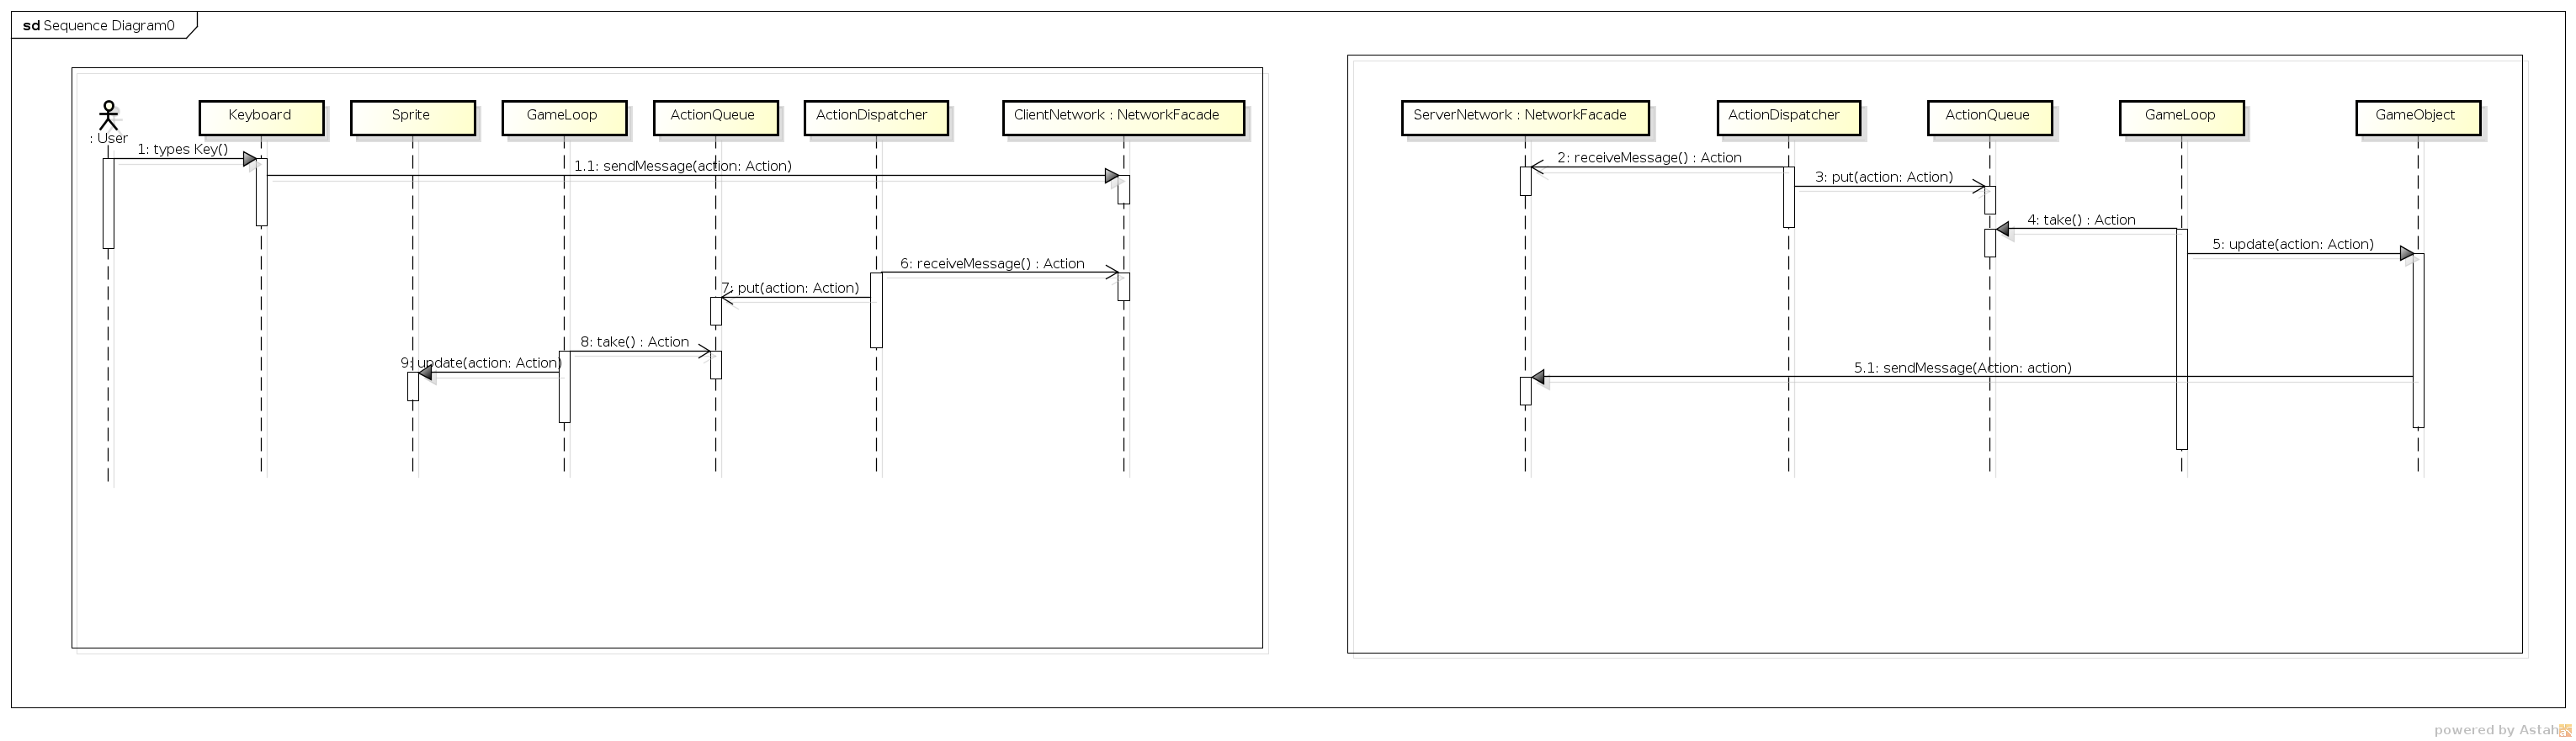
\includegraphics[scale=0.25]{SequenceDiagramAction}
\end{landscape}
\newpage
\section{Logische Architektur: Client}
\subsection{Schnittstellen}
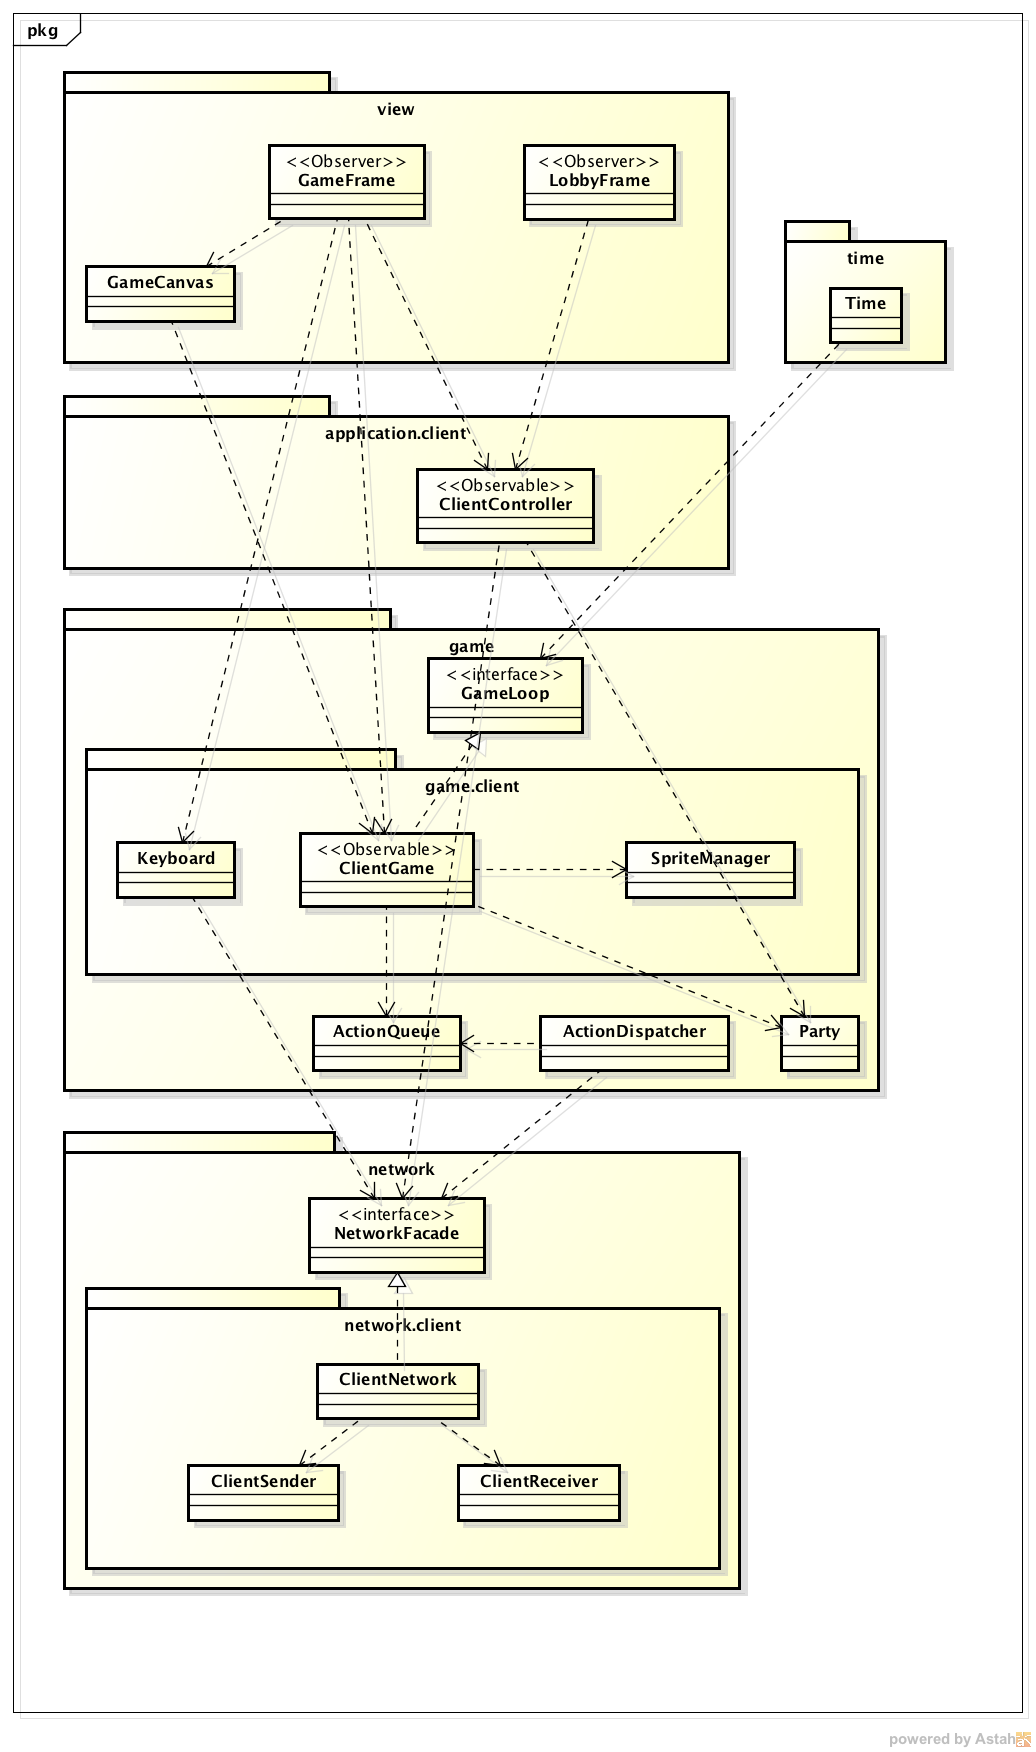
\includegraphics[scale=0.4]{LogischeSichtClient}
\newpage

\subsection{Presentation/view}
Im Package view befinden sich Frames und Canvas, die für die Presentation des Clients notwendig sind.


\subsubsection{Klassenstruktur}
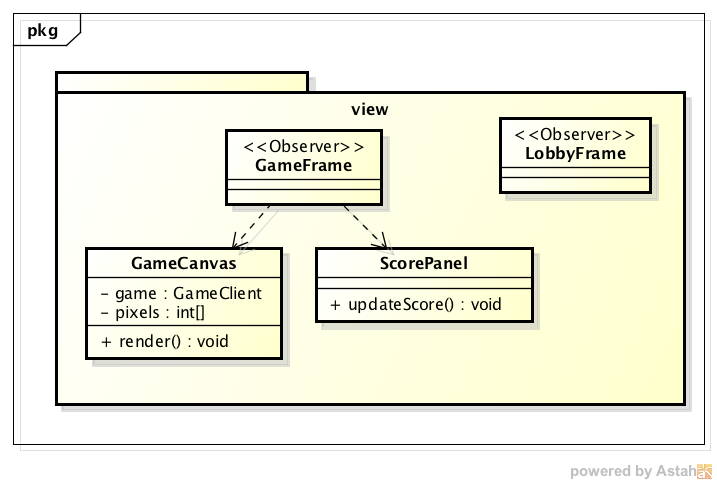
\includegraphics[scale=0.8]{ClassDiagramView}

\textbf{GameCanvas}\\
Der GameCanvas kümmert sich nur um das Rendering, also das Zeichnen der Szene. Dabei delegiert er jedoch nur die pixels[] an alle Sprites, welche sich dann eigenständig zeichnen. Der GameCanvas kümmert sich dann um das performante Buffering.\\

\textbf{ScorePanel}\\
Das ScorePanel zeigt die aktuelle Runde und verbleibende Zeit an. Zudem werden auch die aktuellen Punktestände der einzelnen Spieler dargestellt.\\

\textbf{StartFrame}\\
Das StartFrame übernimmt die Koordination von Connection- und LobbyPanel und zeigt, falls vorhanden, Fehlermeldungen an.\\

\textbf{ConnectionPanel}\\
Im ConnectionPanel wird die Serveradresse eingegeben und der Verbindungsaufbau gestartet.\\

\textbf{LobbyPanel}\\
Das LobbyPanel zeigt alle aktuell am Server angemeldeten Spieler an und deren Status.


\newpage

\subsection{Workflow/application.client}
Im Package application.client befindet sich der workflow des Clients. Er kontrolliert unter anderem wann der LobbyFrame und der GameFrame sichtbar ist.

\subsubsection{Klassenstruktur}
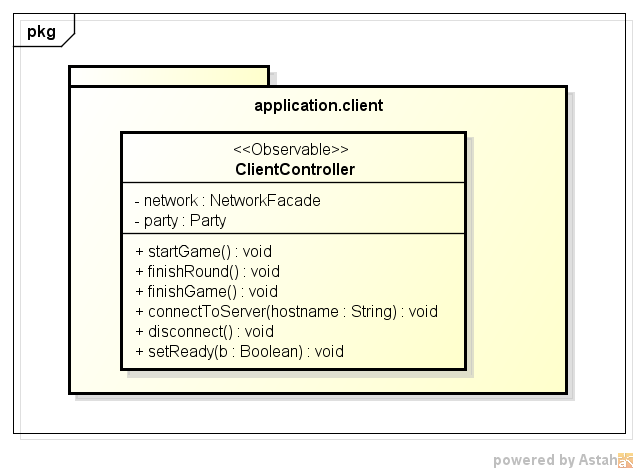
\includegraphics[scale=0.75]{ClassDiagramApplicationClient}
\newpage
\textbf{ClientController}\\
Der ClientController kontrolliert den Zustand der Client-Applikation. Er notifiziert nur den LobbyFrame, nicht aber den GameFrame.\\



\newpage
\subsection{Domain/game.client}
Im Package game.client werden die Actions vom Server interpretiert und die Sprites auf den neusten Stand gebracht. Die Sprites werden in einer Layer-Logik gespeichet, damit sie korrekt gezeichnet werden können.

\subsubsection{Klassenstruktur}
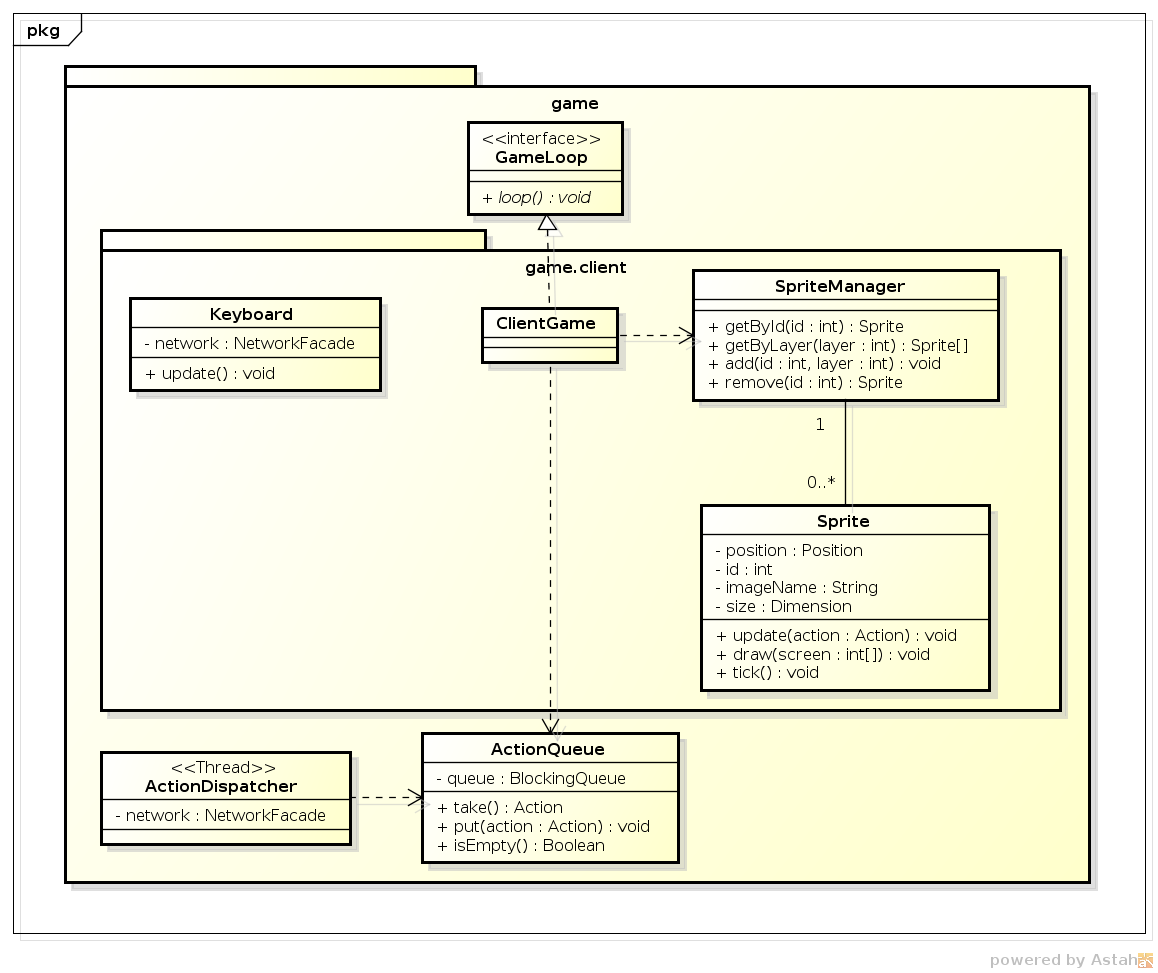
\includegraphics[scale=0.5]{ClassDiagramGameClient}

\textbf{ClientGame}\\
Die Methode loop wird unter "Wichtige Abläufe" beschrieben.\\

\textbf{SpriteManager}\\
Der SpriteManager speicher alle Sprites in einer Schichten-Logik. Dies wird benötig, damit die Sprites korrekt gezeichnet werden können. Zudem können die Sprites per id gefunden werden, damit das aktualisieren der Positionen und Zustände einfacher wird. Die Methoden des SpriteManager sind ähnlich wie bei normalen Datenstrukturen und werden deshalb nicht weiter erläutert.

\newpage

\textbf{Sprite}\\
Die Sprite-Klasse beinhaltet alle Informationen die für das Zeichnen der Spielobjekte benötig wird.\\



\textbf{Keyboard}\\
Das Keyboard zeichnet die Tastatureingaben auf und sendet diese direkt über die Methode update an den Server.

\newpage

\subsection{Network/network.client}

Der Client und der Server implementieren beide das Interface NetworkFacade. Die implementation ist jedoch grundverschieden.

\subsubsection{Klassenstruktur}
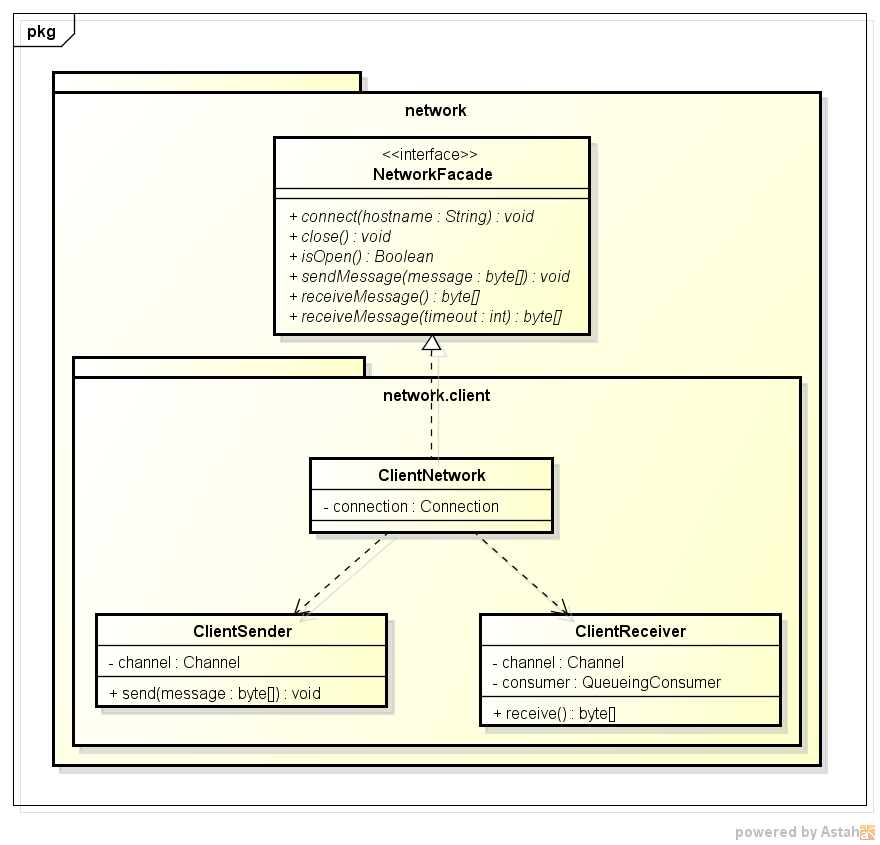
\includegraphics[scale=0.5]{ClassDiagramNetworkClient}

\textbf{ClientNetwork}\\
Die Klasse ClientNetwork implementiert die NetworkFacade.\\

\textbf{ClientSender}\\
Der Client Sender sendet direkt auf eine RabbtiMQ-Queue. Alle Clients senden auf die selbe Queue.\\

\textbf{ClientReceiver}\\
Der ClientReceiver holt Messages aus seiner eigenen RabbitMQ-Queue. Der Server sendet seine Updates auf jede einzelne Queue.

\newpage

\subsection{Wichtige Abläufe}
\subsubsection{Zustandsdiagramm Client Workflow}
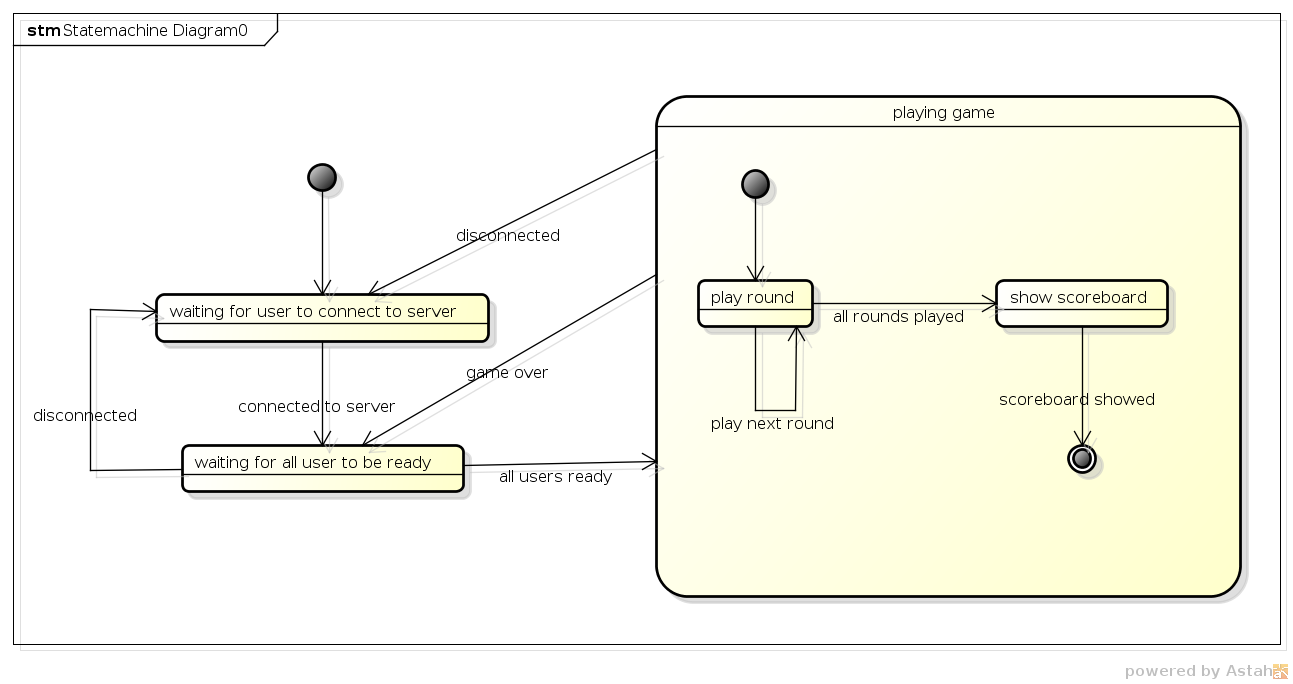
\includegraphics[scale=0.43]{StatemachineClient}

\newpage

\subsubsection{Sequenzdiagramm GameLoop Client}
Das Sequenzdiagramm zeigt nur zwei alternative ActionTypes. Der GameLoop läuft beim Server grundsätzlich gleich ab, jedoch ohne das Rendern und anstelle der Sprites werden mit GameObjects gearbeitet.\\

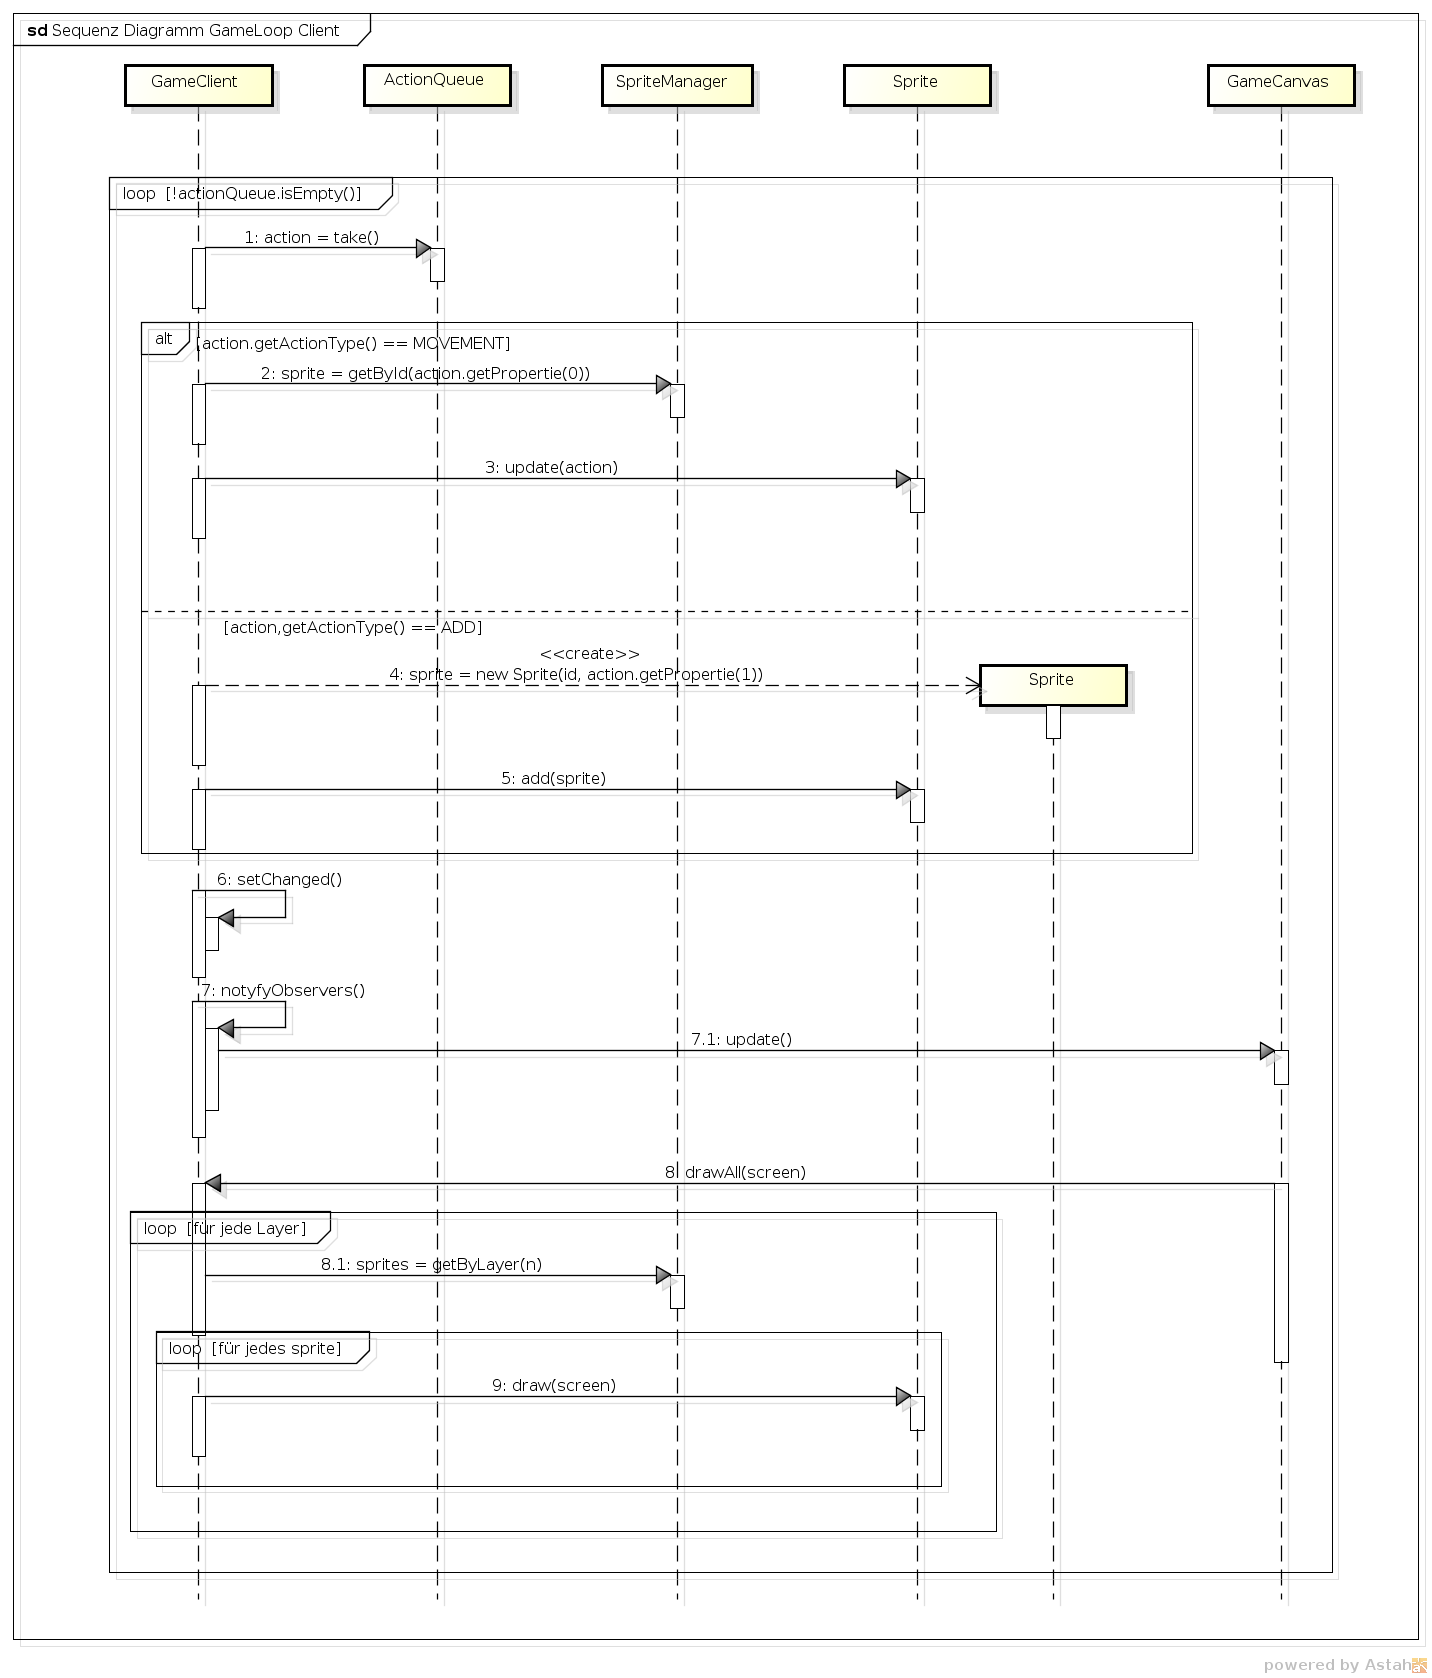
\includegraphics[scale=0.39]{SequenzDiagrammGameLoopClient}
\section{Logische Architektur: Server}
\subsection{Schnittstellen}
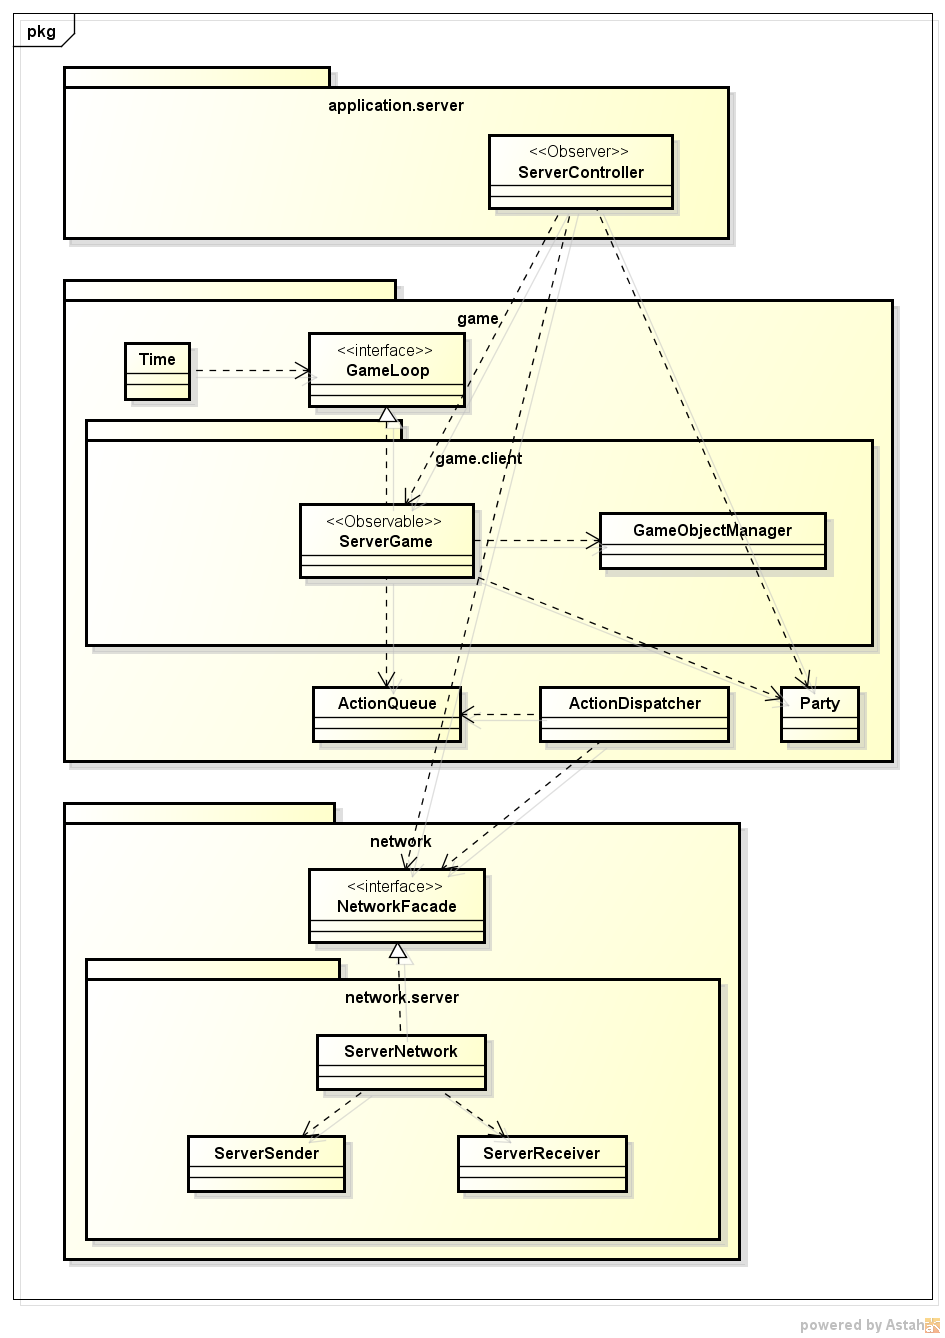
\includegraphics[scale=0.48]{LogischeSichtServer}


\subsection{Workflow/application.server}

Der Workflow des Servers ist sehr simpel. Er wartet bis mehr als zwei Spieler verbunden und bereit sind. Darauf startet der Server dann das Spiel.

\subsubsection{Klassenstruktur}
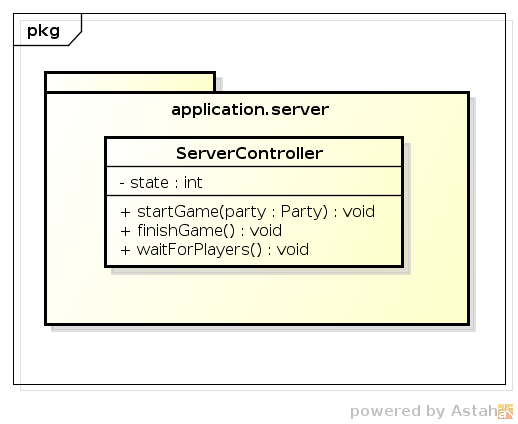
\includegraphics[scale=0.75]{ClassDiagramApplicationServer}


\newpage

\subsection{Domain/game.server}

\subsubsection{Klassenstruktur}
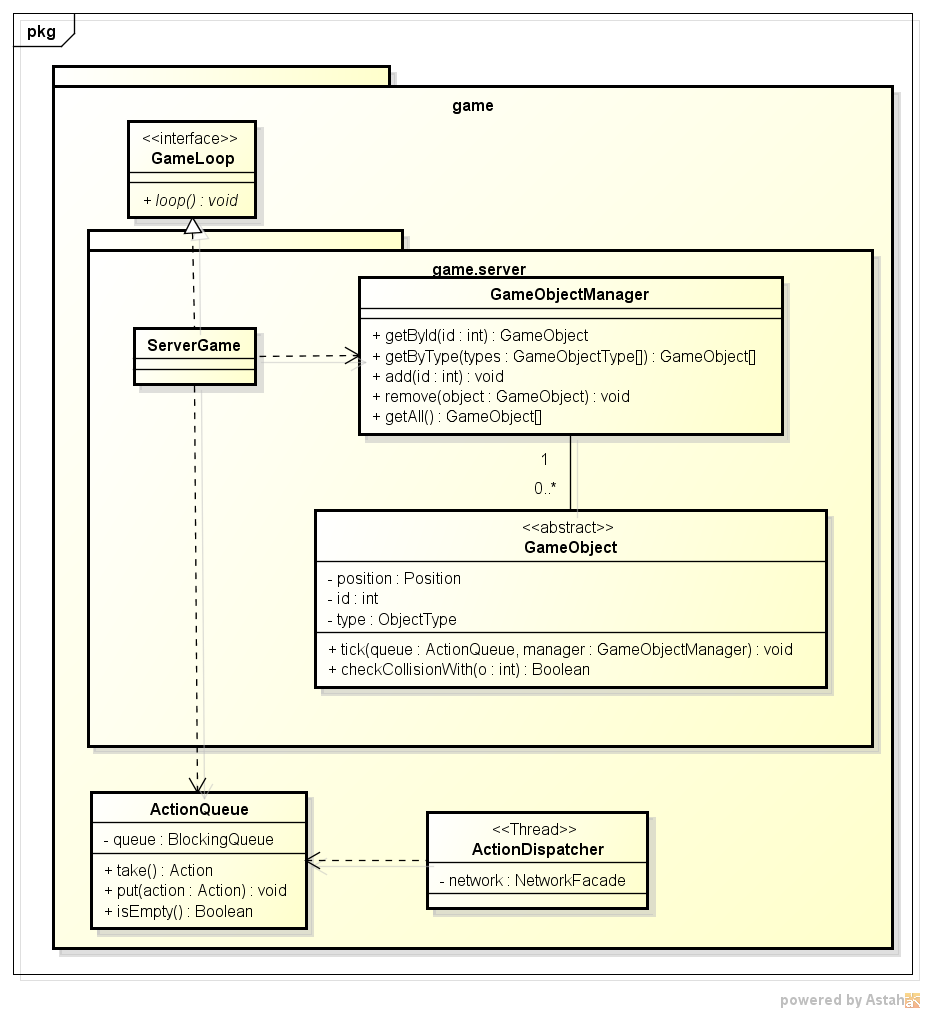
\includegraphics[scale=0.5]{ClassDiagramGameServer}

\textbf{ServerGame}\\
Die Methode loop() funktioniert ähnlich wie die Implementation in der ClientGame Klasse und wurde dort schon beschrieben.\\

\textbf{GameObjectManager}\\
Der GameObjectManager speichert die GameObject nach Typen ab. Dies ist hilfreich, wenn die Objekte aktualisiert werden müssen. Die Methoden des GameObjectManagers sind ähnlich wie bei normalen Datenstrukturen und werden deshalb nicht weiter erläutert.\\

\newpage

\textbf{GameObject}\\
Das GameObject speichert alle nötigen Informationen um das Spielgeschehen und die Interaktionen der Gameobjects zu berechnen.\\

\newpage

\subsection{Network/network.server}

Der Client und der Server implementieren beide das Interface NetworkFacade. Die implementation ist jedoch grundverschieden.

\subsubsection{Klassenstruktur}
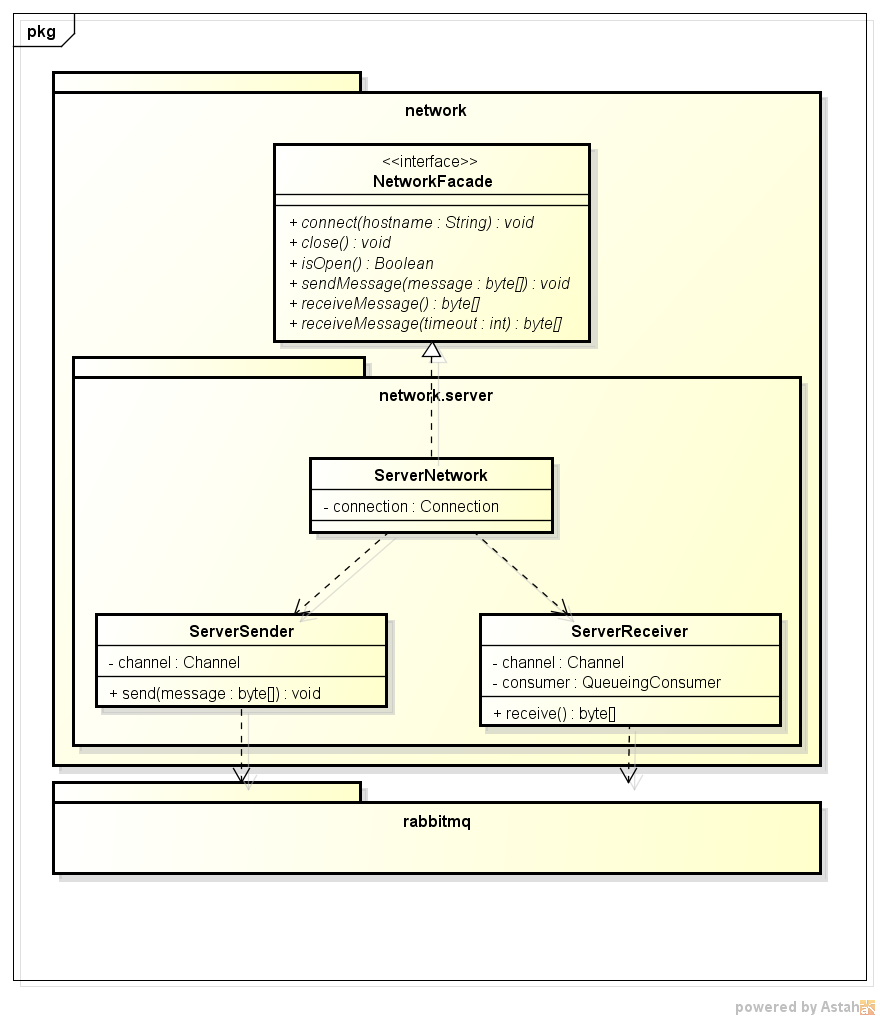
\includegraphics[scale=0.5]{ClassDiagramNetworkServer}

\textbf{ServerNetwork}\\
Die Klasse ServerNetwork implementiert die NetworkFacade.\\

\textbf{ServerSender}\\
Der ServerSender sendet alle Daten die im übergeben werden direkt an alle angemeldeten Clients.\\

\textbf{ServerReceiver}\\
Der ServerReceiver holt alle Daten aus einer einzelnen RabbitMQ-Queue, auf welche alle Clients senden.\\

\newpage

\subsection{Wichtige Abläufe}
\subsubsection{Zustandsdiagramm Server Workflow}
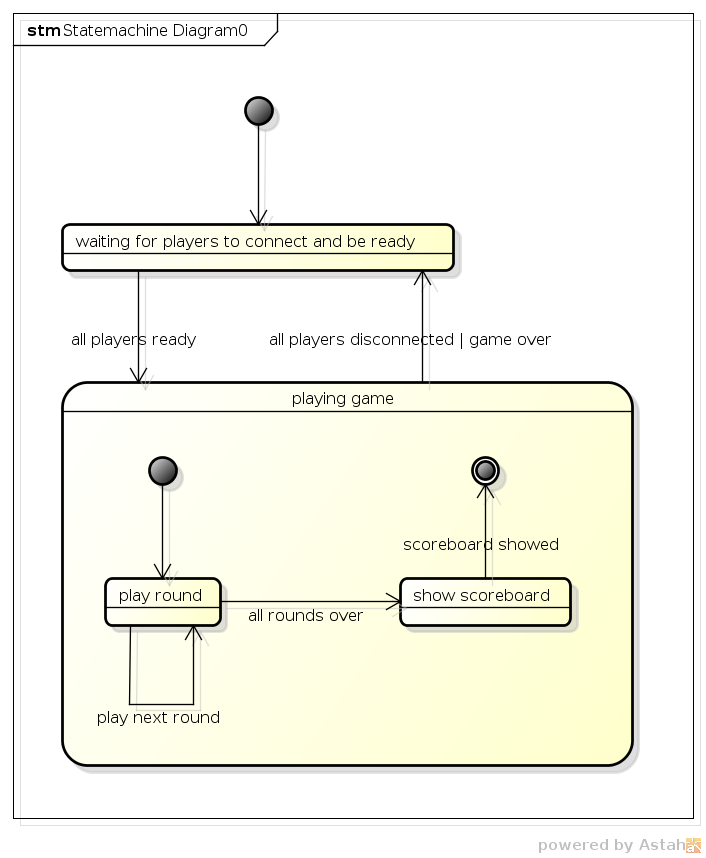
\includegraphics[scale=0.7]{StatemachineServer}

\newpage
 
\section{Prozesse und Threads}
\subsection{Dispatcher Thread}
Der DispatcherThread(Klasse: ActionDispatcher) sorgt dafür, das die Messages empfangen werden und in die ActionQueue abgelegt werden. Gleichzeitig holt der GameLoop die Action aus der Queue heraus. Die ActionQueue ist mittels einer LinkedBlockingQueue implementiert, und somit Threadsafe.\\

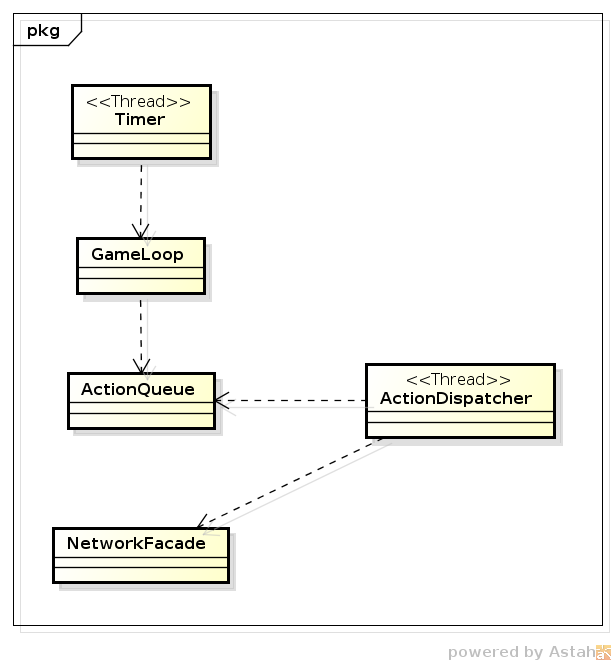
\includegraphics[scale=0.8]{ActionDispatcherProzess}



\newpage

 
\section{Deployment}
Das Messagerouting wird von einem RabbitMQ Broker übernommen, der meistens auf der gleichen Hardware wie der GameServer läuft, aber auch auf einer anderen Hardware betrieben werden kann. Die Übertragung läuft mittels AMQP (Advanced Message Queueing Protocol).\\

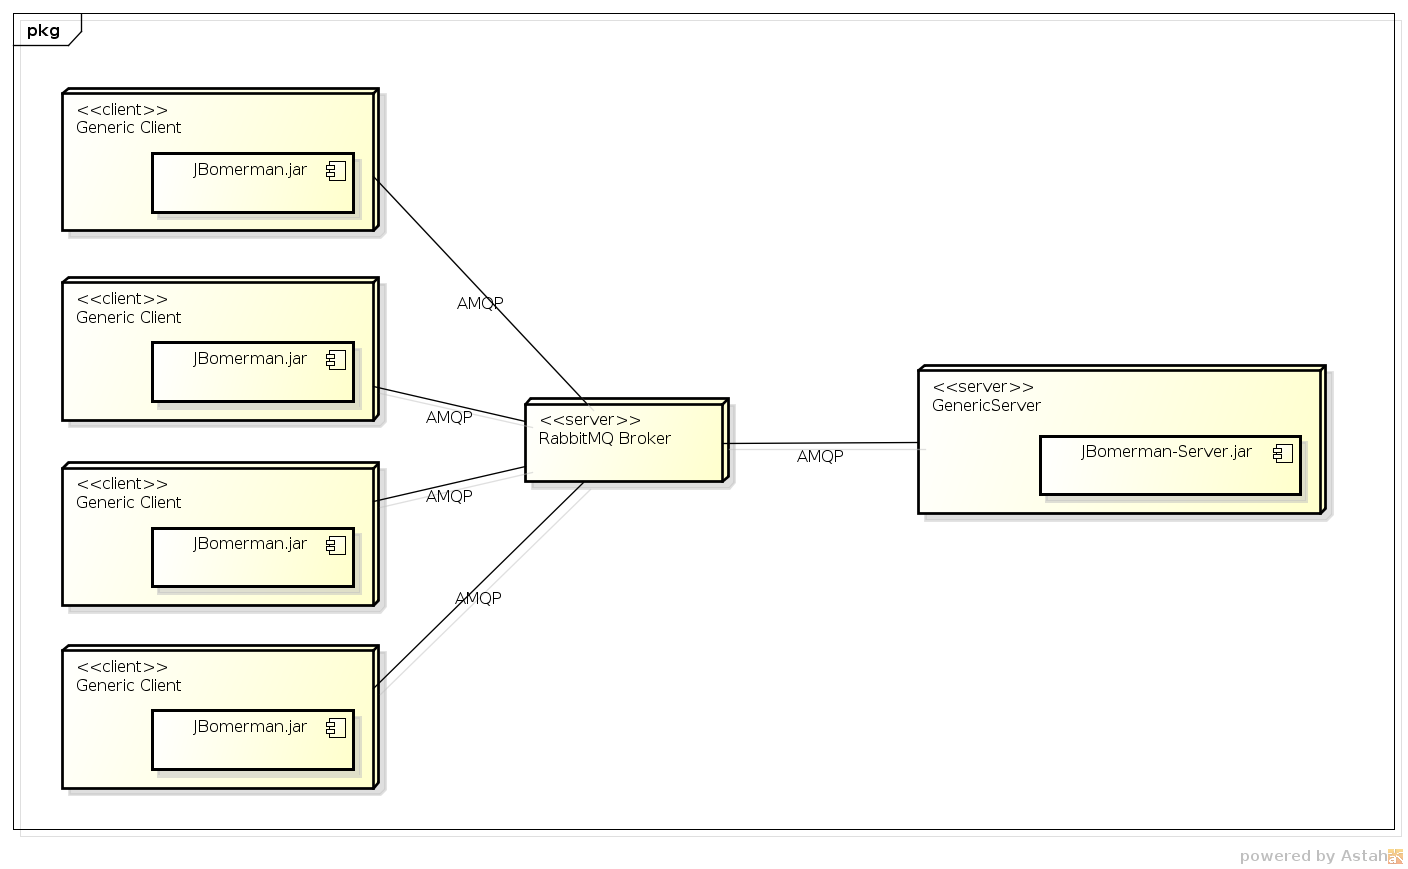
\includegraphics[scale=0.4]{DeploymentDiagram}
 
\newpage

\section{Datenübertragung}
\subsection{RabbitMQ Broker}
Der RabbitMQ Broker speichert die erhaltenen Messages in Warteschlangen/Queues. Der Empfänger muss die Message also nicht sofort annehmen. \\
Die Clients(P) senden ihre Messages an die Queue BombermanInput(hello). Der Server(C) entnimmt dort regelmässig die Messages und kann sie anhand der IDs in den Actions identifizieren.

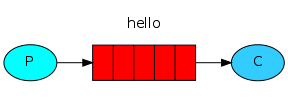
\includegraphics[scale=1.0]{clientToServer}\\\\

Die Messages die vom Server(P) an die Clients(Cx) gehen werden je in eine Client-Eigene Queue(amq.gen-XyZ...) gelegt. Dieser Vorgang übernimmt jedoch der RabbitMQ Broker(X) für uns.

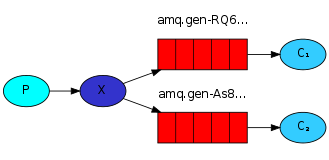
\includegraphics[scale=1.0]{serverToClient}\\

\newpage

\subsection{Actions}
Da die Informationen innerhalb einer Action in einem Object-Array gespeichert werden, müssen die verschiedenen ActionTypen dokumentiert werden.\\

\textbf{MOVEMENT}\\

\begin{tabularx}{\linewidth}{l l l}
\textbf{i} & \textbf{Klasse} & \textbf{Inhalt}\\
\hline
0 & int & id\\
1 & Position & Neue Position\\
2 & BombermanState & Animationsstatus\\
\end{tabularx}\\\\

\textbf{CREATE\_<OBJECTNAME>}\\

\begin{tabularx}{\linewidth}{l l l}
\textbf{i} & \textbf{Klasse} & \textbf{Inhalt}\\
\hline
0 & int & id\\
1 & Position & Anfangsposition\\
\end{tabularx}\\\\

\textbf{DESTROY}\\

\begin{tabularx}{\linewidth}{l l l}
\textbf{i} & \textbf{Klasse} & \textbf{Inhalt}\\
\hline
0 & int & id\\
\end{tabularx}\\\\

\textbf{PLAYER\_INPUT}\\

\begin{tabularx}{\linewidth}{l l l}
\textbf{i} & \textbf{Klasse} & \textbf{Inhalt}\\
\hline
0 & int & id\\
1 & KeyCode & Taste\\
2 & boolean & Taste gedrückt\\
\end{tabularx}\\\\

\textbf{LOBBY\_COMMUNICATION}\\

\begin{tabularx}{\linewidth}{l l l}
	\textbf{i} & \textbf{Klasse} & \textbf{Inhalt}\\
	\hline
	0 & String & Bezeichnung\\
	1...3 & Object & Properties\\
\end{tabularx}\\\\

\textbf{Hinweis: } Weitere Actions werden während der Construction-Phase dokumentiert.

\newpage

\subsection{ControllerCommunication}
Der Actiontype LOBBY\_COMMUNICATION wird für die Kommunikation zwischen Client- und ServerController verwendet. Neben der Bezeichnung werden je nach Message noch folgende Properties übermittelt.\\

\subsubsection{Client to Server}

\textbf{Connect} hat keine weiteren Properties.\\

\textbf{updateState}\\

\begin{tabularx}{\linewidth}{l l l}
	\textbf{i} & \textbf{Klasse} & \textbf{Inhalt}\\
	\hline
	0 & int & PlayerId\\
	1 & boolean & Status (ready / not ready)\\
\end{tabularx}\\\\

\textbf{alive}\\

\begin{tabularx}{\linewidth}{l l l}
	\textbf{i} & \textbf{Klasse} & \textbf{Inhalt}\\
	\hline
	0 & int & PlayerId\\
\end{tabularx}\\\\

\textbf{disconnect}\\

\begin{tabularx}{\linewidth}{l l l}
	\textbf{i} & \textbf{Klasse} & \textbf{Inhalt}\\
	\hline
	0 & int & PlayerId\\
\end{tabularx}\\\\


\subsubsection{Server to Client}
\textbf{ServerFull} hat keine weiteren Properties.\\

\textbf{lobbyList}\\

\begin{tabularx}{\linewidth}{l l l}
	\textbf{i} & \textbf{Klasse} & \textbf{Inhalt}\\
	\hline
	0 & HashMap<Integer, Boolean> & PlayerStates\\
	1 & int & PlayerId\\
\end{tabularx}\\\\

\textbf{updateStates}\\

\begin{tabularx}{\linewidth}{l l l}
	\textbf{i} & \textbf{Klasse} & \textbf{Inhalt}\\
	\hline
	0 & HashMap<Integer, Boolean> & PlayerStates\\
\end{tabularx}\\\\

\textbf{countUpdate}\\

\begin{tabularx}{\linewidth}{l l l}
	\textbf{i} & \textbf{Klasse} & \textbf{Inhalt}\\
	\hline
	0 & int & countdown\\
\end{tabularx}\\\\

\textbf{aliveCheck} hat keine weiteren Properties\\

\textbf{startGame}\\

\begin{tabularx}{\linewidth}{l l l}
	\textbf{i} & \textbf{Klasse} & \textbf{Inhalt}\\
	\hline
	0 & String[][] & Party\\
\end{tabularx}\\\\

\newpage
\section{Externes Design}

Es besteht lediglich ein GUI für den Client, der Server soll über das CLI gestartet werden.
\subsection{StartupFrame}

Als StartupFrame kommt der Connect zum Server,dabei wird die IP oder Name
des Servers benötigt um sich verbinden zu können.
Der Connect Button ist hierbei der Standardbutton.

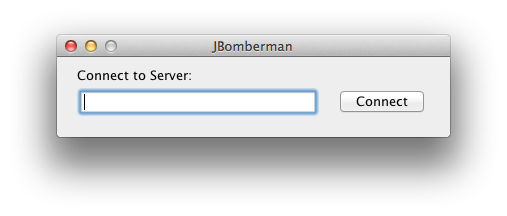
\includegraphics[scale=0.5]{StartupFrame}

\subsection{LobbyFrame}

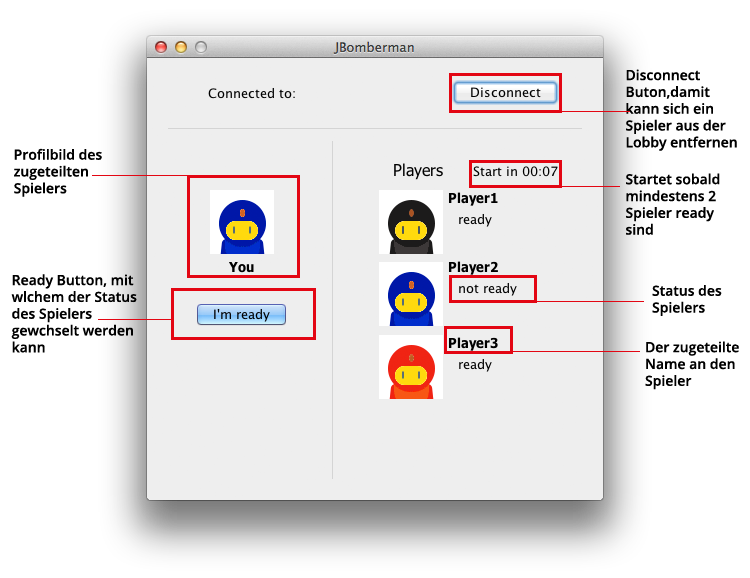
\includegraphics[scale=0.55]{Lobby}


\subsubsection{Fehlermeldungen}
Falls auf dem Server bereits 4 Spieler vorhanden sind wird eine Fehlermeldung 
angezeigt, das der Server bereits Voll ist.

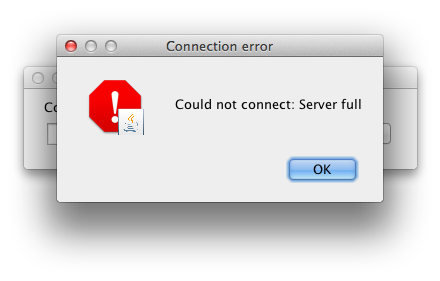
\includegraphics[scale=0.45]{ErrorServerFull}
\newpage
\subsection{GameFrame}
Sobald mindestens 2 Spieler ready waren und er Timer abgelaufen ist startet das 
Spiel.

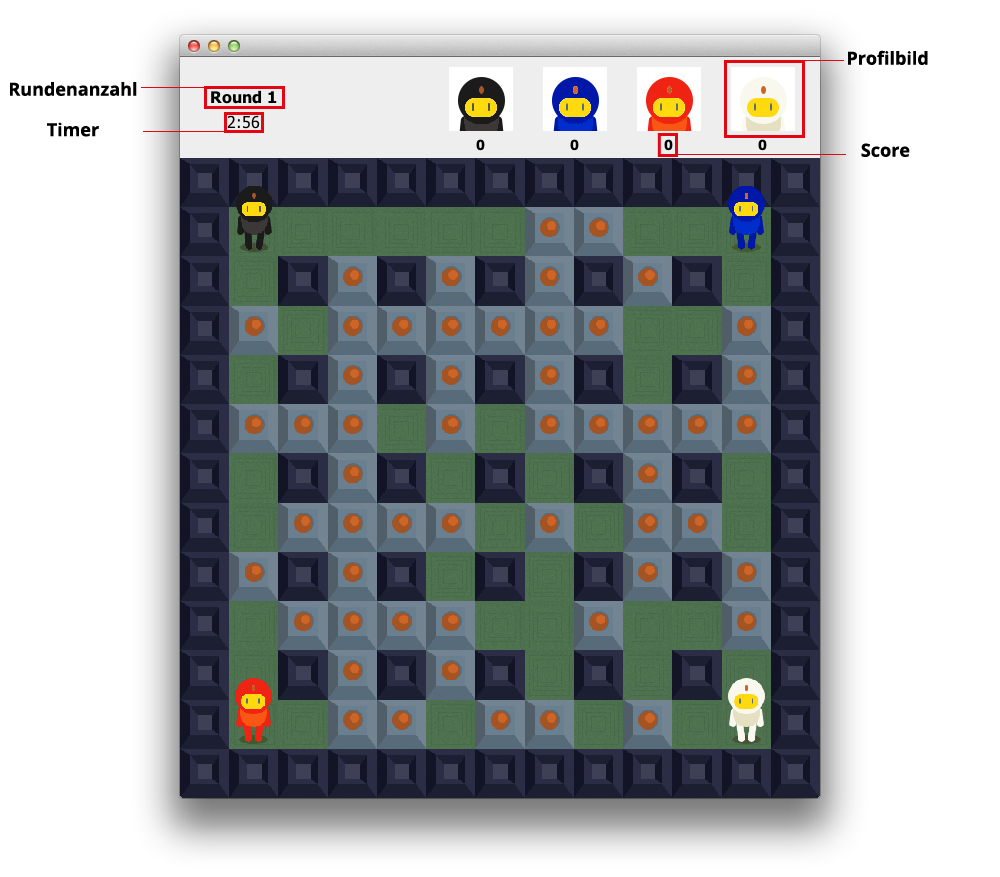
\includegraphics[scale=0.45]{GameFrame}

\section{Grössen und Leistung}
JBomberman wird in zwei einzelne Applikationen unterteilt (Server und Client), dabei werden 
die Sprites auf dem Client gespeichert was diesen natürlich grösser macht ca.: 1 MB. 
Der Server selbst sollte nicht grösser als ca.: 0.5 MB werden.
Das Spiel kann auf allen Clients gespielt werden, welche Java installiert haben 
und eine Tastatur als Eingabegerät haben.
Die Grafiken sind für eine Grösse von 832px x 832px ausgelegt (kann jedoch auch 
verkleinert werden),
 wodurch eigentlich keine minimale Auflösung benötigt wird.

\end{document}